\documentclass[12pt, oneside]{article}

\usepackage[letterpaper, scale=0.89, centering]{geometry}
\usepackage{fancyhdr}
\setlength{\parindent}{0em}
\setlength{\parskip}{1em}

\pagestyle{fancy}
\fancyhf{}
\renewcommand{\headrulewidth}{0pt}
\rfoot{\href{https://creativecommons.org/licenses/by-nc-sa/2.0/}{CC BY-NC-SA 2.0} Version \today~(\thepage)}

\usepackage{amssymb,amsmath,pifont,amsfonts,comment,enumerate,enumitem}
\usepackage{currfile,xstring,hyperref,tabularx,graphicx,wasysym}
\usepackage[labelformat=empty]{caption}
\usepackage[dvipsnames,table]{xcolor}
\usepackage{multicol,multirow,array,listings,tabularx,lastpage,textcomp,booktabs}

\lstnewenvironment{algorithm}[1][] {   
    \lstset{ mathescape=true,
        frame=tB,
        numbers=left, 
        numberstyle=\tiny,
        basicstyle=\rmfamily\scriptsize, 
        keywordstyle=\color{black}\bfseries,
        keywords={,procedure, div, for, to, input, output, return, datatype, function, in, if, else, foreach, while, begin, end, }
        numbers=left,
        xleftmargin=.04\textwidth,
        #1
    }
}
{}
\lstnewenvironment{java}[1][]
{   
    \lstset{
        language=java,
        mathescape=true,
        frame=tB,
        numbers=left, 
        numberstyle=\tiny,
        basicstyle=\ttfamily\scriptsize, 
        keywordstyle=\color{black}\bfseries,
        keywords={, int, double, for, return, if, else, while, }
        numbers=left,
        xleftmargin=.04\textwidth,
        #1
    }
}
{}

\newcommand\abs[1]{\lvert~#1~\rvert}
\newcommand{\st}{\mid}

\newcommand{\A}[0]{\texttt{A}}
\newcommand{\C}[0]{\texttt{C}}
\newcommand{\G}[0]{\texttt{G}}
\newcommand{\U}[0]{\texttt{U}}

\newcommand{\cmark}{\ding{51}}
\newcommand{\xmark}{\ding{55}}

 
\begin{document}
\begin{flushright}
    \StrBefore{\currfilename}{.}
\end{flushright} 
\section*{Monday November 8}
\subsection*{Visualizing induction}


\begin{center}
    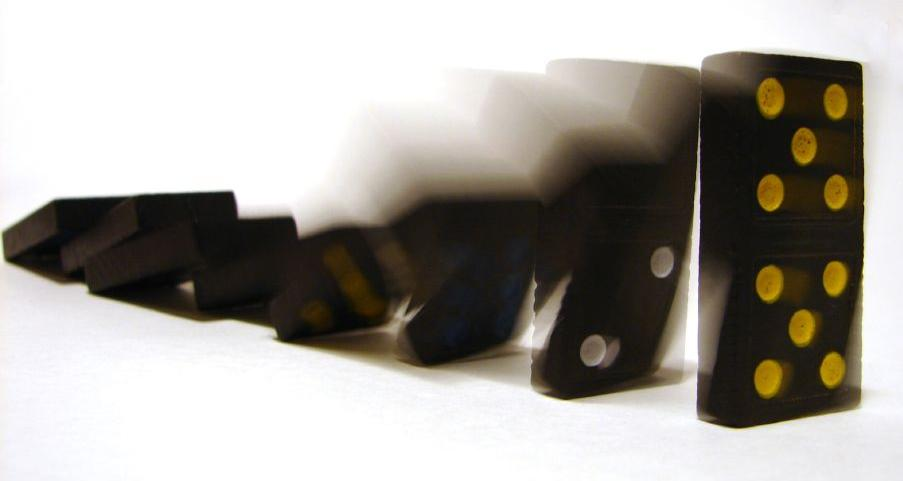
\includegraphics[width=2in]{../../resources/images/Domino_Cascade.jpeg}

    {\tiny Wikimedia commons\\ \href{https://creativecommons.org/licenses/by/2.0/legalcode}{https://creativecommons.org/licenses/by/2.0/legalcode} }
\end{center} 

\fbox{\parbox{\textwidth}{

{\bf Proof by Mathematical Induction}

To prove a universal quantification over the set of all integers greater than
or  equal to some  base integer $b$,

\vspace{-10pt}

\begin{itemize}
\item[] {\bf Basis Step}:  Show the property holds for $b$. 
\item[]  {\bf Recursive Step}:  Consider an arbitrary integer $n$ greater than or  equal to  $b$, assume
    (as the {\bf induction hypothesis})  that the property holds  for $n$, and use  this and
    other facts to  prove that  the property holds for $n+1$.
\end{itemize}

}} 

\fbox{\parbox{\textwidth}{

{\bf Proof by Strong Induction}

To prove that a universal quantification over the set of all integers greater than or equal to some  base integer $b$ holds,  pick a  fixed nonnegative integer  $j$ and then: \hfill 

\begin{tabularx}{\textwidth}{lX}
    {\bf Basis Step}: & Show the statement holds for $b$, $b+1$, \ldots, $b+j$. \\
    {\bf Recursive Step}: & Consider an arbitrary integer $n$ greater than or  equal to $b+j$, assume
    (as the {\bf strong  induction hypothesis})  that the property holds  for {\bf each of} $b$, $b+1$, \ldots, $n$, 	
    and use  this and
    other facts to  prove that  the property holds for $n+1$.
\end{tabularx}
}} 
 \newpage


{\bf Theorem}: Every positive integer is a sum of (one or more) distinct powers of $2$.
{\it Binary expansions exist!}

Recall the definition for binary expansion:



{\bf Definition} For $n$ a positive integer, 
the {\bf binary expansion of $n$}  is
\[
(a_{k-1} \cdots a_1 a_0)_b
\]
where $k$ is a positive integer, $a_0, a_1, \ldots, a_{k-1}$ 
are each $0$ or $1$, $a_{k-1} \neq  0$, and
\[
n =  \sum_{i=0}^{k-1} a_{i} b^{i}
\]
 

The idea in the ``Least significant first" algorithm 
for computing binary expansions is that the binary
expansion of {\it half} a number becomes {\it part} of the binary expansion of 
the number of itself. We can use this 
idea in a proof by strong induction that binary expansions exist for all 
positive integers $n$.


{\bf Proof by strong induction}, with $b=1$ and $j=0$.


{\bf Basis step}:  WTS property is true about  $1$.

\phantom{Choose $a_0 = 1$, then $(a_0)_2 = 1 \cdot 2^0 = 1$.}
\vspace{80pt}


{\bf Recursive step}: Consider an arbitrary integer $n \geq 1$.

Assume (as the strong induction hypothesis, IH) that the property is true about  each of $1, \ldots, n$.  

WTS that the property is true about $n+1$.

{\it Idea}: We will apply the IH to $(n+1) \textbf{ div } 2$.

{\it Why is this ok?}

\phantom{Notice that $(n+1) \textbf{ div } 2$ is greater than or equal to 
$1$ and less than or equal to $n$ because $n \geq 1$.}
\vspace{100pt}

{\it Why is this helpful?}

By the IH, we can write $(n+1) \textbf{ div } 2$ as 
a sum of powers of $2$. In other words, 
there are values $a_{k-1}, \ldots, a_0$ such that each $a_i$ is $0$ or $1$, $a_{k-1} = 1$, 
and
\[
    \sum_{i=0}^{k-1} a_i 2^i = (n+1) \textbf{ div } 2   
\]
Define the collection of coefficients
\[
   c_{j} = 
   \begin{cases}
        a_{j-1} \qquad&\text{if $1 \leq j \leq k$}\\
        (n+1) \textbf{ mod } 2 &\text{if $j = 0$}
   \end{cases}
\]
Calculating: 
\begin{alignat*}{2}
    \sum_{j=0}^k c_j 2^j &= c_0 + \sum_{j=1}^k c_j 2^j 
    = c_0 + \sum_{i=0}^{k-1} c_{i+1} 2^{i+1} &\qquad &\text{re-indexing the summation}\\
    &= c_0 + 2 \cdot \sum_{i=0}^{k-1} c_{i+1}2^i &\qquad &\text{factoring out a $2$ from each term in the sum}\\
    &= c_0 + 2 \cdot \sum_{i=0}^{k-1} a_{i} 2^i &\qquad &\text{by definition of $c_{i+1}$}\\
    &= c_0 + 2 \left(~(n+1) \textbf{ div } 2 ~\right) &\qquad &\text{by IH} \\
    &= \left(~ (n+1) \textbf{ mod } 2 ~\right ) + 2 \left(~(n+1) \textbf{ div } 2 ~\right) &\qquad &\text{by definition of $c_0$} \\
    &= n+1 &\qquad&\text{by definition of long division}
\end{alignat*}

Thus, $n+1$ can be expressed as a sum of powers of $2$, as required. 
\subsubsection*{Representing positive integers with primes}


{\bf Theorem}: Every positive integer {\it greater than 1} is a product of (one or more) primes.

{\bf Before we prove, let's try some examples}:

$20 = $

$100 = $

$5 = $


{\bf Proof by strong induction}, with $b=2$ and $j=0$.

{\bf Basis step}:  WTS property is true about  $2$.

Since $2$ is itself prime,
it is already written as a product of (one) prime.


{\bf Recursive step}: Consider an arbitrary integer $n \geq 2$.
Assume (as the strong induction hypothesis, IH) that the property is true about  each of $2, \ldots, n$.  
WTS that the property is true about  $n+1$: We want to show that $n+1$ can be written 
as a product of primes.  Notice that $n+1$ is itself prime or it is composite.

{\it Case 1}: assume $n+1$ is prime and then immediately it is written as a product
of (one) prime so we are done.  

{\it Case 2}: assume that $n+1$ is composite
so there are integers $x$ and $y$ where $n+1 = xy$ and each of them is between $2$ and $n$
(inclusive).  Therefore, the induction hypothesis applies to each of $x$ and $y$ so each 
of these factors of $n+1$ can be written as a product of primes.  Multiplying these products together, 
we get a product of primes that gives $n+1$, as required. 

Since both cases give the necessary
conclusion, the proof by cases for the recursive step is complete. \subsubsection*{Sending old-fashioned mail with postage stamps}


Suppose we had postage stamps worth $5$ cents and $3$ cents.
Which number of cents can we form using these stamps?
In other words, which postage can we pay?

$11$? 

$15$? 


$4$?



\begin{align*}
    &CanPay(0) \land \lnot CanPay(1) \land \lnot CanPay(2) \land \\
    &CanPay(3) \land \lnot CanPay(4) \land CanPay(5) \land CanPay(6) \\
    &\lnot CanPay(7) \land \forall n \in \mathbb{Z}^{\geq 8} CanPay(n)
\end{align*}

where the predicate $CanPay$ with domain $\mathbb{N}$ is
\[
    CanPay(n) = \exists x \in \mathbb{N} \exists y \in \mathbb{N}  ( 5x+3y = n)
\]


{\bf Proof} (idea): First, explicitly give witnesses or general arguments
for postages between $0$ and $7$. 
To prove the universal claim, we can use mathematical induction or strong induction.

{\it Approach 1, mathematical induction}: if we have
stamps that add up to $n$ cents, need to use them (and others)
to give $n+1$ cents. How do we get $1$ cent with just $3$-cent
and $5$-cent stamps?

\vspace{-10pt}
Either \underline{take away a $5$-cent stamps and add two $3$-cent stamps},

\vspace{-10pt}
or \underline{take away three $3$-cent stamps and add two $5$-cent stamps}.

\vspace{-10pt}
The details of this proof by mathematical induction
are making sure we have enough 
stamps to use one of these approaches.

{\it Approach 2, strong induction}: assuming we know how to make postage
for {\bf all} smaller values (greater than or equal to $8$), when
we need to make $n+1$ cents, \underline{add one $3$ cent stamp to 
however we make $(n+1) - 3$ cents}.

\vspace{-10pt}
The details of this proof by strong induction are making sure we 
stay in the domain of the universal when applying the induction hypothesis.
 \newpage
\subsection*{Review}
\begin{enumerate}
    \item \hspace{1in} \\ 

In class, we proved the theorem that: 
Every positive integer is a sum of (one or more) distinct powers of $2$.

What's wrong with the following {\it attempted} proof of this fact?


{\bf Attempted proof by mathematical induction}, with $b=1$.

{\bf Basis step}: WTS $1$ can be written 
as a sum of (one or more) distinct powers of $2$. Since $1 =2^0$, 
we are done.

{\bf Recursive step}: Consider an arbitrary integer $n \geq 1$.
By the IH, we can write $n$ as a sum of distinct powers of $2$.
Since $1 = 2^0$, it is a power of $2$ and we can add it as a term 
to this sum of powers of $2$. When we do so, the terms sum to $n+1$
and we are done.

\begin{enumerate}
\item The basis step is not sufficient.
\item The induction hypothesis is not stated correctly.
\item It's wrong to say that $1$ is a power of $2$.
\item Adding the $2^0$ to the sum of powers doesn't give the correct value.
\item Adding the $2^0$ to the sum of powers 
is problematic for a different reason.
\end{enumerate}
     \item \hspace{1in}\\ 


Recall that a prime factorization is a product of primes (potentially with some of the primes
occurring more than once).
Select all and only the correct prime factorizations of positive integers.

\begin{enumerate}
    \item $2\cdot 2 \cdot 2 \cdot 2$
    \item $3$
    \item $3 \cdot 4 \cdot 5$
    \item $17 \cdot 21$
    \item $2 \cdot 11$
\end{enumerate}     \newpage
    \item 

In this question, we'll consider two possible 
proofs of the statement
\[
    \forall n  \in  \mathbb{Z}^{\geq 8}  \exists x \in \mathbb{N}  \exists y \in \mathbb{N}  (  5x+3y =  n)
\]

\begin{enumerate}
\item First approach, using mathematical induction ($b=8$).

{\bf Basis step}:  WTS property is true about $8$.
Consider the witnesses $x = 1$, $y=1$. These 
are nonnegative integers and $5 \cdot 1 + 3 \cdot 1 = 8$, as
required.

{\bf Recursive step}: Consider an  arbitrary  $n \geq 8$.
Assume (as the induction hypothesis, IH) that there are nonnegative integers
$x, y$ such that $n =  5x +  3y$.  WTS
that there are nonnegative integers $x', y'$ such
that  $n+1 = 5x' +  3y'$.  We consider two cases, 
depending on  whether  any  $5$ cent stamps
are used for $n$.

{\it Case 1}:  Assume $x \geq  1$ (we assume that at least one
$5$ cent stamp is used for $n$).
Define $x' = x-1$ and $y'=y+2$ (both in  $\mathbb{N}$ by case assumption).


Calculating:
\begin{align*}
5x' +  3y' &\overset{\text{by def}}{=}  5(x-1) +  3(y+2)  = 5x -  5 +3y +   6  \\
&\overset{\text{rearranging}} = (5x+3y) -5  + 6\\
& \overset{\text{IH}}{=} n-5+6 =  n+1
\end{align*}


{\it  Case 2}: Assume $x = 0$.  Therefore  $n  = 3y$,  so 
since  $n \geq 8$, $y \geq 3$. Define $x' = 2$ and $y'=y-3$
(both in $\mathbb{N}$ by case assumption).
Calculating:
\begin{align*}
5x' +  3y' &\overset{\text{by def}}{=}  5(2) +  3(y-3)  = 10  +3y -9  \\
&\overset{\text{rearranging}} = 3y +10 -9 \\
&\overset{\text{IH and case}}{=} n+10-9 =  n+1
\end{align*}

Since the goal has been proved from each case, the proof by cases is complete and
we have proved the recursive step. $\square$\\


Why was the recursive step split into two cases?
\begin{enumerate}
    \item Because there are two variables $x$ and $y$ that need witnesses.
    \item Because the statement has alternating quantifiers $\forall$ and $\exists$
    \item Because the witness values need to be nonnegative and subtraction may lead to negative values.
    \item Because the domain is all integers greater than or equal to $8$.
    \item Because there are two steps in the recursive definition of $\mathbb{N}$
\end{enumerate}

\item  Second approach, by strong induction ($b=8$ and $j=2$)

{\bf Basis step}:  WTS property is true about  $8, 9, 10$
\begin{itemize}
\item Consider the witnesses $x = 1$, $y=1$. These 
are nonnegative integers and $5 \cdot 1 + 3 \cdot 1 = 8$, as
required.
\item Consider the witnesses $x = 0$, $y=3$. These 
are nonnegative integers and $5 \cdot 0 + 3 \cdot 3 = 9$, as
required.
\item Consider the witnesses $x = 2$, $y=0$. These 
are nonnegative integers and $5 \cdot 2 + 3 \cdot 0 = 10$, as
required.
\end{itemize}

{\bf Recursive step}: Consider an  arbitrary  $n \geq 10$.
Assume, as the strong induction hypothesis, 
that the property is true about each of $8, 9, 10, \ldots, n$.  
WTS
that there are nonnegative integers $x', y'$ such
that  $n+1 = 5x' +  3y'$. 

Since \underline{Blank 1}, 
by the strong induction hypothesis, there are nonnegative integers
$x, y$ such that $(n+1) - 3 = 5x + 3y$.
Choosing \underline{Blank 2} works because
\[
    5x' + 3y' = 5x + 3y + 3 = (n+1) - 3 + 3 = n+1.
\]

Choose a true and useful statement to fill in Blank 1.
    \begin{enumerate}
        \item $n \geq 10$ and hence $(n+1) - 3 \geq 8$
        \item $n \geq 8$ and hence $(n+1)-3 \geq 8$
        \item $n \geq 8$ and hence $(n+1) \geq 9$
    \end{enumerate}

Choose the appropriate statement to fill in Blank 2.
    \begin{enumerate}
        \item $x' = x, y' = y$
        \item $x' = x+1, y' = y+1$
        \item $x' = x+1, y' = y$
        \item $x' = x, y' = y+1$
        \item $x' = x-1, y' = y-1$
        \item $x' = x-1, y' = y$
        \item $x' = x, y' = y-1$
    \end{enumerate}
\end{enumerate}
 \end{enumerate}

\newpage
\section*{Wednesday November 10}

\subsubsection*{Finding a winning strategy for a game}


Consider the following game: two players start with 
two (equal) piles of jellybeans in front of them.
They take turns removing any positive integer number
of jellybeans at a time from one of two piles in 
front of them in turns.

The player who removes the last jellybean wins the game.

Which player (if any) has a strategy to guarantee
to win the game?


Try out some games, starting with $1$ jellybean in each pile,
then $2$ jellybeans in each pile, then $3$ jellybeans in each pile.
Who wins in each game?

\vspace{200pt}


Notice that reasoning about the strategy for the $1$ jellybean 
game is easier than about the strategy for the $2$ jellybean game.

{\it Formulate a winning strategy by working to 
transform the game to a simpler one we know we can win.}

\newpage

{\it Player 2's Strategy}: Take the same number of jellybeans that Player 1 did, 
but from the opposite pile. 


{\it Why is this a good idea}: If Player 2 plays this strategy, at the next turn
Player 1 faces a game with the same setup as the original, just with fewer
jellybeans in the two piles. Then Player 2 can keep playing this strategy to win.

{\bf Claim}: Player 2's strategy guarantees they will win the game.

{\bf Proof}: By strong induction, we will prove that for all positive 
integers $n$, Player 2's strategy guarantees a win in the game that starts with 
$n$ jellybeans in each pile.

{\bf Basis step}: WTS Player 2's strategy guarantees a win 
when each pile starts with $1$ jellybean.

In this case, Player 1 has to take the jellybean from one of the piles
(because they can't take from both piles at once).
Following the strategy, Player 2 takes the jellybean from the 
other pile, and wins because this is the last jellybean.

{\bf Recursive step}: Let $n$ be a positive integer. 
As the strong induction hypothesis, assume that
Player 2's strategy guarantees a win in the games 
where there are $1, 2, \ldots, n$ many jellybeans in each 
pile at the start of the game.

WTS that Player 2's strategy guarantees a win in the game where
there are $n+1$ in the jellybeans in each pile at the start of the game.

In this game, the first move has Player 1 take 
some number, call it $c$ (where $1 \leq c \leq n+1$),
of jellybeans from one of the piles. 
Playing according to their strategy, Player 2 then 
takes the same number of jellybeans from  the other pile.

Notice that $(c = n+1) \lor (c \leq n)$.

{\it Case 1}: Assume $c = n+1$, then in their first move, 
Player 2 wins because they take all of the second pile, which 
includes the last jellybean.

{\it Case 2}: Assume $c \leq n$. Then after Player 2's first move,
the two piles have an equal number of jellybeans. The number
of jellybeans in each pile is 
\[
    (n+1) - c
\]
and, since $1 \leq c \leq n$, this number is between $1$ and $n$.
Thus, at this stage of the game, the game appears identical to a new 
game where the two piles have an equal number of jellybeans between $1$
and $n$. Thus, the strong induction hypothesis applies, and Player 2's
strategy guarantees they win.

 \newpage


\fbox{\parbox{\textwidth}{

{\bf New! Proof by Contradiction} 

To prove that a statement $p$ is true, pick another statement $r$ and once we show
that $\neg p  \to (r \wedge  \neg r)$ then  we can conclude that  $p$ is  true.

{\it Informally} The statement we care about can't possibly be false, so it must be true.
}} 

 \subsection*{Least and greatest}


For a set of numbers $X$, how do you formalize ``there is a greatest $X$'' 
or ``there is a least $X$''?

\vspace{30pt}

{\bf Prove} or {\bf  disprove}:  There is a least prime number.

\vspace{100pt}

{\bf Prove} or {\bf  disprove}: There is a greatest integer. 

{\it Approach 1, De Morgan's and universal generalization}: 

\vspace{100pt}

{\it Approach 2, proof by contradiction}: 

\vspace{200pt}

{\it Extra examples}: 
Prove or disprove that $\mathbb{N}$,  $\mathbb{Q}$ each have a
least and a greatest element. 
 
\newpage
\subsection*{Review}
\begin{enumerate}
\item \hspace{1in}\\ 

Recall the game Nim from class.

\begin{enumerate}
    \item Why did we use strong induction to prove that Player 2's strategy guarantees a win?
    \begin{enumerate}
        \item Because there are two players in the game.
        \item Because each turn can involve a player taking some positive number 
        of jellybeans from a pile, not just one jellybean.
        \item Because the strategy player 2 uses depends on what player 1 does.
        \item Because the set of natural numbers is recursively defined.
    \end{enumerate}
    \item  If we modify the game so that in each turn, a player could take jellybeans
    from one or both piles, which player has a winning strategy?
    \begin{enumerate}
        \item Player 1.
        \item Player 2.
        \item Neither in general, the existence of a winning strategy for the players depends 
        on how many jellybeans are in each pile to start.
    \end{enumerate}
    \item  If we modify the game so that in each turn, a player must take 
    exactly one jellybean, which player has a winning strategy?
    \begin{enumerate}
        \item Player 1.
        \item Player 2.
        \item Neither in general, the existence of a winning strategy for the players depends 
        on how many jellybeans are in each pile to start.
    \end{enumerate}
\end{enumerate}
 \item \hspace{1in}\\ 

We will prove that there is no greatest prime number

{\bf Proof} Assume, towards a \underline{BLANK1}, that 
there is a greatest prime number, call it $n_{BIG}$.
In particular, this means that there are finitely many 
primes. Let's label them in order $p_1, \ldots, p_n$ where 
$p_1 = 2$ and $p_n = n_{BIG}$.
Choose $r = $ \underline{BLANK2}. We proved in class
that $r$ is {\bf true}. It remains to show that (under our 
assumption) $r$ is {\bf false}, because
that would complete the contradiction argument.
Define the integer
\[
    C = (p_1 \cdots p_n) + 1
\]
This is a positive integer greater than $1$. 
However, we will show that it does not have any prime
factors and thus is not a product of primes.
By our assumption, the only prime numbers are $p_1, \ldots, 
p_n$. Thus, to show that $C$ does not have any prime
factors means to show that $p_i$ is not a factor 
of $C$ for each value of $i$ from $1$ to $n$. 
Towards a universal generalization, let $i$ be an arbitrary
between $1$ and $n$ (inclusive). We need to prove that $p_i$ is 
not a factor of $C$. By definition of $C$,
\[
    C = p_i ( p_1 \cdots p_{i-1} p_{i+1} \cdots p_n) + 1
\]
so $C \textbf{ div } p_i = p_1 \cdots p_{i-1} p_{i+1} \cdots p_n$
and $C \textbf{ mod } p_i = 1$ (because $p_i > 1$ since it is prime).
Since $C \textbf{ mod } p_i \neq 0$, $p_i$ is not a factor of $C$.
Thus $C$ witnesses that the universal claim is false, 
and we have proved that $r$ is false.




\begin{enumerate}
\item BLANK1
    \begin{enumerate}
        \item universal generalization
        \item proof of existential by witness
        \item direct proof
        \item proof by contrapositive
        \item proof by cases
        \item proof by contradiction
    \end{enumerate}
\item BLANK2
\begin{enumerate}
    \item The least prime number is $2$.
    \item There is a greatest prime number.
    \item There is a least prime number.
    \item Every positive integer greater than $1$ is a product of primes.
    \item Every positive integer has a base expansion.
    \item There is a greatest integer.
    \item There is no greatest integer.
\end{enumerate}
\end{enumerate} \item \hspace{1in}\\ 

Select all and only the situations in which the given
proof strategy would be available.

\begin{enumerate}
\item When might it be appropriate to use induction?
    \begin{enumerate}
        \item To prove that an existential claim over the set of integers is true.
        \item To prove that a universal claim over the real numbers is true.
        \item To prove that a conditional claim is true.
        \item None of the above.
    \end{enumerate}
\item When might it be appropriate to use proof by contradiction?
    \begin{enumerate}
        \item To prove that an existential claim over the set of integers is true.
        \item To prove that a universal claim over the real numbers is true.
        \item To prove that a conditional claim is true.
        \item None of the above.
    \end{enumerate}
\end{enumerate}
 \end{enumerate}

\newpage
\section*{Friday November 12}



{\bf Definition}: {\bf Greatest common divisor} Let $a$ and $b$ be integers, not both zero. The largest integer $d$ such that 
$d$ is a  factor of $a$ and $d$ is a factor of  $b$ is called the greatest common divisor of $a$ and $b$ 
and is denoted by $gcd(~(a, b)~)$. 

Why do we restrict to the situation where $a$ and $b$ are not both zero?

\vspace{50pt}


Calculate $gcd(~(10,15)~)$

\vspace{50pt}

Calculate $gcd(~(10,20)~)$

\vspace{50pt} 

{\bf Claim}: For any integers $a,b$ (not both zero), $gcd(~(a,b)~) \geq 1$.

{\bf Proof}: {\it Show that $1$ is a common factor of any two integers, so since the gcd 
is the greatest common factor it is greater than or equal to any common factor.}

\vspace{150pt}

{\bf Claim}: For any positive integers $a,b$, $gcd(~(a,b)~) \leq a$ and $gcd( ~(a,b)~) \leq b$.

{\bf Proof} {\it Using the definition of gcd and the fact that factors of a positive integer
are less than or equal to that integer.}

\vspace{150pt}

{\bf Claim}: For any positive integers $a,b$, if $a$ divides $b$ then $gcd(~(a,b)~) = a$.

{\bf Proof} {\it Using previous claim and definition of gcd.}

\vspace{150pt}


{\bf Claim}: For any positive integers $a,b,c$, if there is some integer $q$ such that $a = bq + c$,
\[
    gcd(~(a,b)~) = gcd (~(b,c)~)
\]
{\bf Proof} {\it Prove that any common divisor of $a,b$ divides $c$ and that any common 
divisor of $b,c$ divides $a$.}

\vspace{150pt}
 

{\bf Lemma}: For any integers $p, q$ (not both zero), 
$gcd \left(~ \left(~\frac{p}{gcd(~(p,q)~)}, \frac{q}{gcd(~(p,q)~)} ~\right) ~\right) = 1$ .
In other words, can reduce to relatively prime integers by dividing by gcd.

{\bf Proof}:

Let $x$ be arbitrary positive integer and assume that $x$ is a 
factor of each of $\frac{p}{gcd(~(p,q)~)}$ and $\frac{q}{gcd(~(p,q)~)}$. 
This gives integers $\alpha$, $\beta$ such that 
\[
    \alpha x = \frac{p}{gcd(~(p,q)~)} \qquad \qquad \beta x = \frac{q}{gcd(~(p,q)~)}
\]
Multiplying both sides by the denominator in the RHS: 
\[
    \alpha x \cdot gcd(~(p,q)~)= p \qquad \qquad \beta x \cdot gcd(~(p,q)~)= q
\]
In other words, $x \cdot gcd(~(p,q)~)$ is a common divisor of $p, q$. By definition of $gcd$, this means
\[
    x \cdot gcd (~(p,q)~) \leq gcd (~(p,q)~)
\]
and since $gcd(~(p,q)~)$ is positive, this means, $x \leq 1$.
\vspace{350pt}
 
\newpage
\subsection*{Sets of numbers}

We've seen multiple representations of the set of positive integers
(using base expansions and using prime factorization). Now we're 
going to expand our attention to other sets of numbers as well.


The {\bf set  of rational numbers}, $\mathbb{Q}$  is defined as 
\[
\left\{ \frac{p}{q} \mid p \in \mathbb{Z}  \text{ and  } q  \in \mathbb{Z} \text{ and } q \neq  0 \right\}
\text{~~~~or, equivalently,~~~~}
\{ x  \in  \mathbb{R} \mid \exists p \in \mathbb{Z}  \exists q \in \mathbb{Z}^+ ( p =  x \cdot q) \}
\]

{\it Extra practice}: Use the definition of set equality to prove that the definitions above  give the same set.

 

We have the following subset relationships between sets of numbers:

\[
    \mathbb{Z}^{+} \subsetneq \mathbb{N} \subsetneq \mathbb{Z} \subsetneq \mathbb{Q} \subsetneq \mathbb{R}
\]


Which of the proper subset inclusions above can you prove?

\vspace{50pt} 

{\bf Goal}:  The square root of $2$ is not a rational number.  In other words: $\neg \exists x \in \mathbb{Q} ( x^2 -  2 = 0)$

{\bf Attempted proof}: The definition of the set of rational numbers is the collection of fractions $p/q$ where $p$ is an integer and $q$ is a nonzero integer. Looking for a {\bf witness} $p$ and $q$, we can write the square root of $2$ as the fraction 
$\sqrt{2 }/1$, where $1$ is a nonzero integer. Since the numerator is not in the domain, this witness is not allowed, and we have shown that the square root of $2$ is not a fraction of integers (with nonzero denominator). Thus, the square root of $2$ is not rational.


{\it The problem in the above attempted proof is that} \underline{\phantom{it only considers one candidate witness
and does not prove that no witnesses exist.}}


{\bf Lemma 1:} For every two integers $a$ and  $b$, not both zero, with  $gcd(~(a,b)~) = 1$, it is not the case that both $a$
is  even and $b$ is even.


{\bf Lemma 2:} For every integer  $x$, $x$ is  even if and only if $x^2$  is even.


{\bf Proof}: Towards a proof by contradiction, we will define a statement 
$r$ such that $\sqrt{2} \in \mathbb{Q} \to (r \land \lnot r)$. 

Assume that $\sqrt{2} \in \mathbb{Q}$. Namely, there are positive integers
$p, q$ such that 
\[
    \sqrt{2} = \frac{p}{q}
\]
Let $a= \frac{p}{gcd( ~(p,q)~)}$, $b = \frac{q}{gcd(~(p,q)~)}$, then 
\[
    \sqrt{2} = \frac{a}{b} \qquad \text{and} \qquad gcd(~(a,b)~) = 1
\]

By Lemma 1, $a$ and $b$ are not both even. We define $r$ to be the 
statement ``$a$ is even and $b$ is even'', and we have proved $\lnot r$.

Squaring both sides and clearing denominator: $2b^2 = a^2$.

By definition of even, since $b^2$ is an integer$, a^2$ is even.

By Lemma 2, this guarantees that $a$ is even too. So, by 
definition of even, there is some integer (call it $c$), such that $a = 2c$.

Plugging into the equation:
\[
    2b^2 = a^2 = (2c)^2 = 4c^2
\]
and dividing both sides by $2$
\[
    b^2 = 2c^2
\]
and since $c^2$ is an integer, $b^2$ is even. By Lemma 2, $b$ is even too.
Thus, $a$ is even and $b$ is even and we have proved $r$. 

In other words, assuming that $\sqrt{2} \in \mathbb{Q}$ guarantees $r \land \lnot r$, 
which is impossible, so $\sqrt{2} \notin \mathbb{Q}$. QED

 
\newpage
\subsection*{Review}
\begin{enumerate}
\item \hspace{1in}\\ 

We will consider two ways for calculating the gcd. In each 
part of the question, you'll calculate $gcd(~(306, 120)~$).

\begin{enumerate}
\item The first approach uses some of the claims we proved in class
to get the following algorithm:


\begin{algorithm}[caption={Euclidean algorithm for calculating greatest common divisor}]
    procedure $\textit{Euclidean}$($a$: a positive integer, $b$: a positive integer)
    $x$ := $a$
    $y$ := $b$
    while $y \neq 0$
      $r$ := $x \textbf{ mod } y$
      $x$ := $y$
      $y$ := $r$
    return $x$ $\{ \textrm{the result of } gcd(~(a,b)~)\} $
\end{algorithm} 
Tracing this algorithm, lines 2 and 3 initialize the variables 
\[
    x:= 306 \qquad y:=120
\]
Entering the while loop, the variable $r$ is initialized to
\[
    r:= 66
\]
because $306 = 2 \cdot 120 + 66$ so $306 \textbf{ mod } 120 = 66$.
Calculate and fill in the updated value of $r$ in each subsequent iteration
of the {\bf while} loop, and then give the value of $gcd(~(306, 120)~$).

\item The second approach uses the representation of positive integers
greater than $1$ as products of primes. To calculate $gcd(~(a,b)~)$ we 
find the prime factorizations of each of $a$ and $b$, and then calculate
the number that results from multiplying together terms $p^c$ where $p$ is 
a prime that appears in {\it both} prime factorizations of $a$ and $b$
and $c$ is the {\it minimum} number of times $p$ appears in the two factorizations.

Select the prime factorizations for $306$ and $120$ and express their 
$gcd$ as a product of powers of primes.

Possible factorizations:
\begin{enumerate}
        \item $306 = 2 \cdot 153$, $120 = 2 \cdot 60$
        \item $306 = 1 \cdot 2 \cdot 3 \cdot 3 \cdot 17$, $120 = 1 \cdot 3 \cdot 5 \cdot 8$
        \item $306 = 2 \cdot 3 \cdot 3 \cdot 17$, $120 = 2 \cdot 2 \cdot 2 \cdot 3 \cdot 5$
\end{enumerate}

Possible $gcd$ choices:
\begin{enumerate}
\item $2$
\item $2 \cdot 3$
\item $5 \cdot 17$
\item $2^3 \cdot 3^2$
\item $2^3 \cdot 3^2 \cdot 5 \cdot 8 \cdot 17$
\end{enumerate}
\end{enumerate} \newpage
\item \hspace{1in}\\ 

{\it Goals for this question: recognize that we can prove the same statement
in different ways.  Trace proofs and justify why they are valid.}

Below are two proofs of the same statement: fill in the blanks with the 
expressions below.

{\bf Claimed statement}:  \textbf{(a)}$\underline{\phantom{\hspace{1.3in}}}$
\begin{quote}

{\bf Proof 1}: Using De Morgan's law for quantifiers, 
we can rewrite this statement as a universal of the negation of the body of the statement.
Towards a proof by universal generalization, let $x$ be an arbitrary element of $\mathbb{Z}$. Then we need to show that
$$\textbf{(b)}\underline{\phantom{\hspace{1.3in}}}$$

We proceed by contradiction to show that $$(x \textrm{ is odd} \land x^2 \textrm{ is even}) \to \textbf{(c)}\underline{\phantom{\hspace{1.3in}}}$$
We assume by direct proof that $(x \textrm{ is odd} \land x^2 \textrm{ is even})$. Then, $(x^2 \textrm{ is even})$ follows directly from this assumption, so by definition 
of conjunction, we must show that $(x^2 \textrm{ is not even})$ to complete the proof.
From the assumption, we have that $(x \textrm{ is odd})$.  Applying the definition of odd, $x = 2k + 1$ for some $k \in \mathbb{Z}$. Then $x^2 = 4k^2 + 4k + 1$. We can rewrite the right hand side to $2(2k^2 + 2k) + 1$. This shows that $x^2$ is odd by the definition of odd, since choosing $j = 2k^2 + 2k$ gives us $j \in \mathbb{Z}$ with $x^2 = 2j + 1$. Since a number is either even or odd and not both, and $x^2$ is odd, then it must not be even. 
This concludes the proof, as we have assumed the negation of the original statement and deduced a contradiction
from this assumption.
\end{quote}

\newpage
\begin{quote}{\bf Proof 2}: 

    \begin{tabular}{l p{2.5in}}
    1. \begin{tabular}{l}
        \textbf{To Show} $\forall x \in \mathbb{Z} \neg (x \textrm{ is odd} \land x^2 \textrm{ is even})$\\
    \end{tabular}
    & Rewriting statement using De Morgan's law for quantifiers
 \\ 
   2. \begin{tabular}{l}
        \textbf{Choose arbitrary} $x \in\mathbb{Z}$ \\
        \textbf{To Show} \textbf{(d)}$\underline{\phantom{\hspace{1.3in}}}$\\
    \end{tabular}
    & By \textbf{(e)}$\underline{\phantom{\hspace{1.3in}}}$\\
 \\
    3. \begin{tabular}{l}
        \textbf{To Show}
         $x \textrm{ is odd} \to \neg  (x^2 \textrm{ is even})$
    \end{tabular}
    & Rewrite previous {\bf To Show} using logical equivalence
    \\
    4. \begin{tabular}{l}
        \textbf{Assume } $x \textrm{ is odd}$ \\
        \textbf{To Show } $\neg  (x^2 \textrm{ is even})$ \\
    \end{tabular}
    & By \textbf{(f)}$\underline{\phantom{\hspace{1.3in}}}$\\
    \\    
    5. \begin{tabular}{l}
        \textbf{To Show} $x^2 \textrm{ is odd}$
    \end{tabular}
    & Rewrite previous {\bf To Show} using definition of even, odd
    \\
    6. \begin{tabular}{l}
        \textbf{Use the witness} $k$, an integer,\\
        where $x = 2k+1$\\
    \end{tabular}
     & By existential definition of $x$ being odd \\
    \\
    7. \begin{tabular}{l}
        \textbf{Choose the witness} \\
        $j = 2k^2 + 2k$, an integer\\
        \textbf{To Show} $x^2 = 2j+1$
    \end{tabular}
     & Show this new {\bf To Show} is true to prove the existential definition of $x^2$ being odd\\
    \\
    8.\begin{tabular}{l}
        \textbf{To Show} $(2k+1)^2  = 2j+1$
    \end{tabular}
    & Rewrite previous {\bf To Show} using definition of $k$
    \\
    9.  \begin{tabular}{l}
        \textbf{To Show} $(2k+1)^2  = 2(2k^2 + 2k) + 1$
    \end{tabular}
    & Rewrite previous {\bf To Show} using definition of $j$
    \\
    10. \begin{tabular}{l}
        \textbf{To Show } $T$ \\
    \end{tabular}
     & By algebra: multiplying out the LHS; factoring the RHS\\
    QED & Because we got to $T$ only by rewriting \textbf{To Show} to equivalent statements, using valid proof techniques and definitions. \\
    \end{tabular}
\end{quote}


Consider the following expressions as options to fill in the two proofs above. Give your answer as one of the numbers below for each blank a-c. You may use some numbers for more than one blank, but each letter only uses one of the expressions below.

\begin{multicols}{2}
\begin{enumerate}[label=\roman*.]
    \item $\exists x \in \mathbb{Z} \, (x \textrm{ is odd} \land x^2 \textrm{ is even})$
    \item $\neg \exists x \in \mathbb{Z} \, (x \textrm{ is odd} \land x^2 \textrm{ is even})$
    \item $\exists x \in \mathbb{Z} \, (x \textrm{ is odd} \land x \textrm{ is even})$
    \item $\neg \exists x \in \mathbb{Z} \, (x \textrm{ is odd} \land x \textrm{ is even})$
    \item $\exists x \in \mathbb{Z} \, (x^2 \textrm{ is odd} \land x^2 \textrm{ is even})$
    \item $\neg \exists x \in \mathbb{Z} \, (x^2 \textrm{ is odd} \land x^2 \textrm{ is even})$
    \item $(x^2 \textrm{ is even} \land x^2 \textrm{ is not even})$
    \item $\neg (x \textrm{ is odd} \land  x^2 \textrm{ is even})$
    \item $(x \textrm{ is odd} \land  x^2 \textrm{ is even})$
    \item $(x \textrm{ is odd} \land  x \textrm{ is not odd})$
    \item $\neg (x \textrm{ is odd} \land  x \textrm{ is not odd})$
    \item $x^2 \textrm{ is even}$
    \item $x^2 \textrm{ is odd}$
    \item universal generalization
    \item proof by cases
    \item direct proof
    \item proof by contraposition
    \item proof by contradiction
\end{enumerate}
\end{multicols}
 \end{enumerate}

\end{document}